\chapter{バリデーション}
\label{validation}
\section{概要}
制作された修士作品が実際にはどのように体験されるのかについて調査した。

\section{実施方法}
\subsection{Video Cued-Recall メソッド}
本作品を評価する上では、体験時、体験者がどのようなことに注意を向け、どのような行動を取ったかについて精緻に振り返る必要がある。そのため本研究では、Video Cued-Recallという手法を用いて体験時の言語データの収集を行なった。 Video Cued-Recallとは、体験時のようすが記録された映像を視聴しながら、体験者本人が映像を手がかりに作品での体験を回顧し、言語化する方法である\cite{Costello2005}。インタビューを通して回顧するよりも詳細に体験を振り返ることができ、また体験しているそのときに体験のようすについて語ってもらう方法よりも、自然な体験について記述できることがその利点として挙げられる。

\subsection{参加者について}
インタビューは、愛知県名古屋市のファブ施設であるFabCafe Nagoyaでの展示に際して、本作品に関する予備知識のない4名の体験者を対象に実施した。ただし、うち1名(参加者4)は「Relation」の体験時、トラッキングの精度が著しく低下していたため、1つ目に体験した「Familiar / Strange」の体験についてのみ調査の対象とした。

\begin{figure}[H]
  \centering
  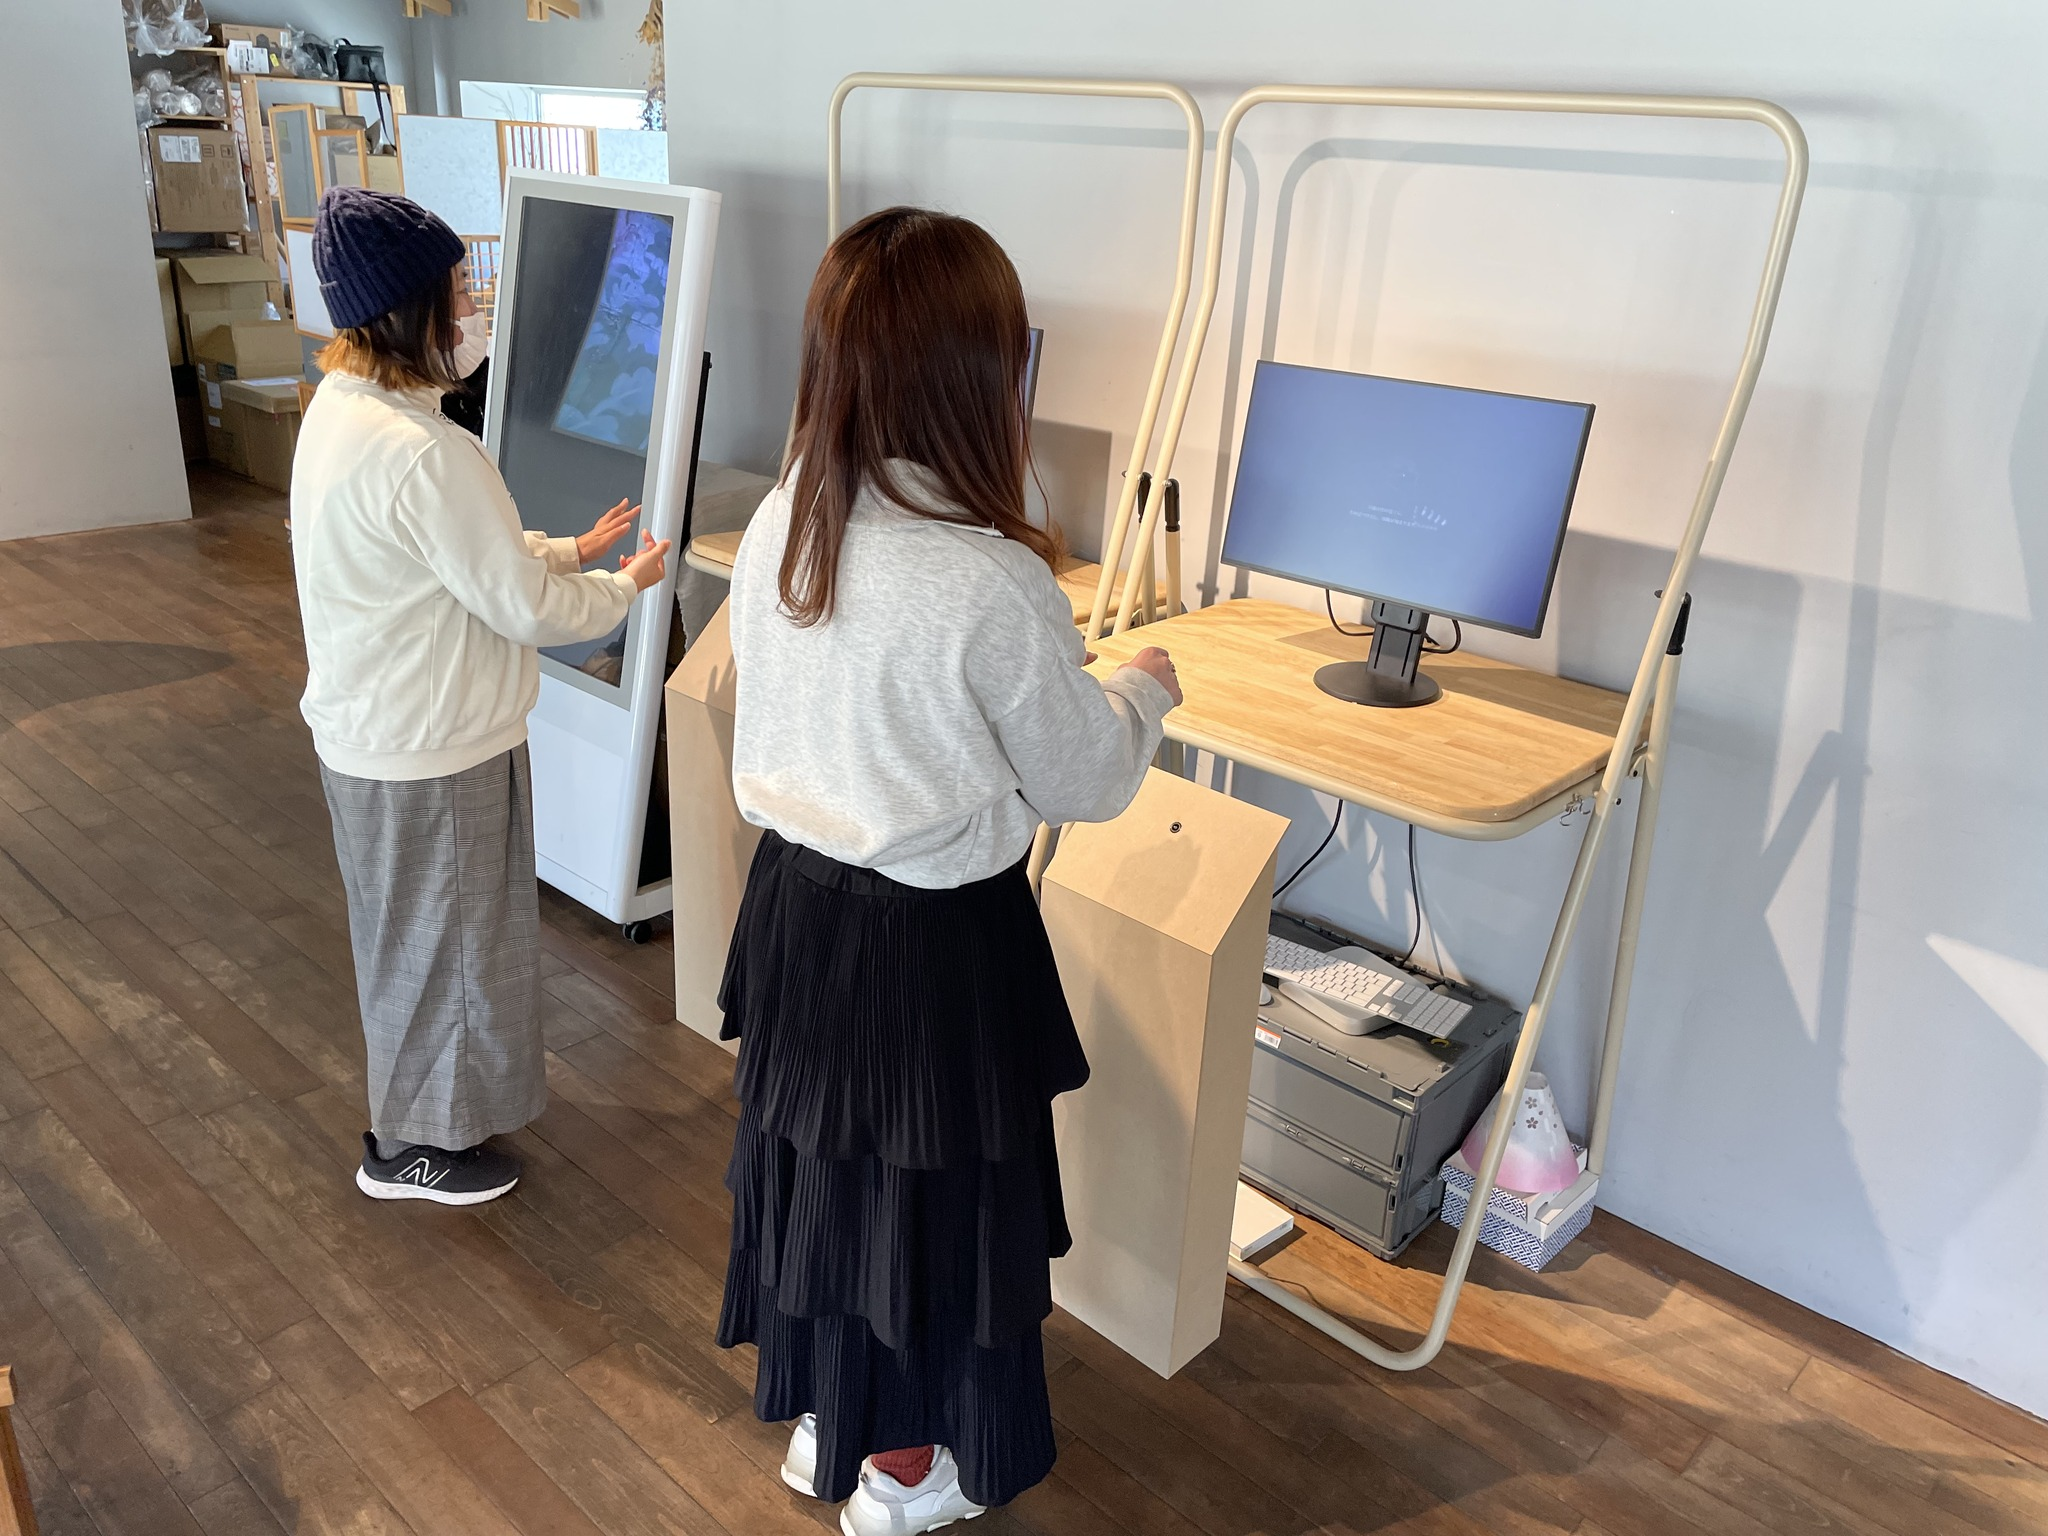
\includegraphics[width=10cm]{img/exhibit_at_fabcafe.jpeg}
  \caption{FabCafe Nagoyaでの展示}
  \label{fig:exhibit_at_fabcafe}
\end{figure}

\subsection{データ収集}
参加者にはまず、調査の大まかな流れについて説明し、撮影についての許諾を得た。コンセプトの説明が自然な体験に影響することを避けるため、作品の体験の前にはコンセプトや具体的な作品の内容については説明せず、トラッキングされた手が次々に形を変えていくこと、手の形が表示された状態から始まり、再びもとの手の形に戻るループ構造のある作品であること、という最低限の構造のみ伝えた。

体験のようすは、手もとのハンドトラッキングを行うカメラ映像、現在時刻、体験者が実際に見ているスクリーンの映像が図\ref{fig:record_monitor}のようにレイアウトされて記録される。

\begin{figure}[H]
  \centering
  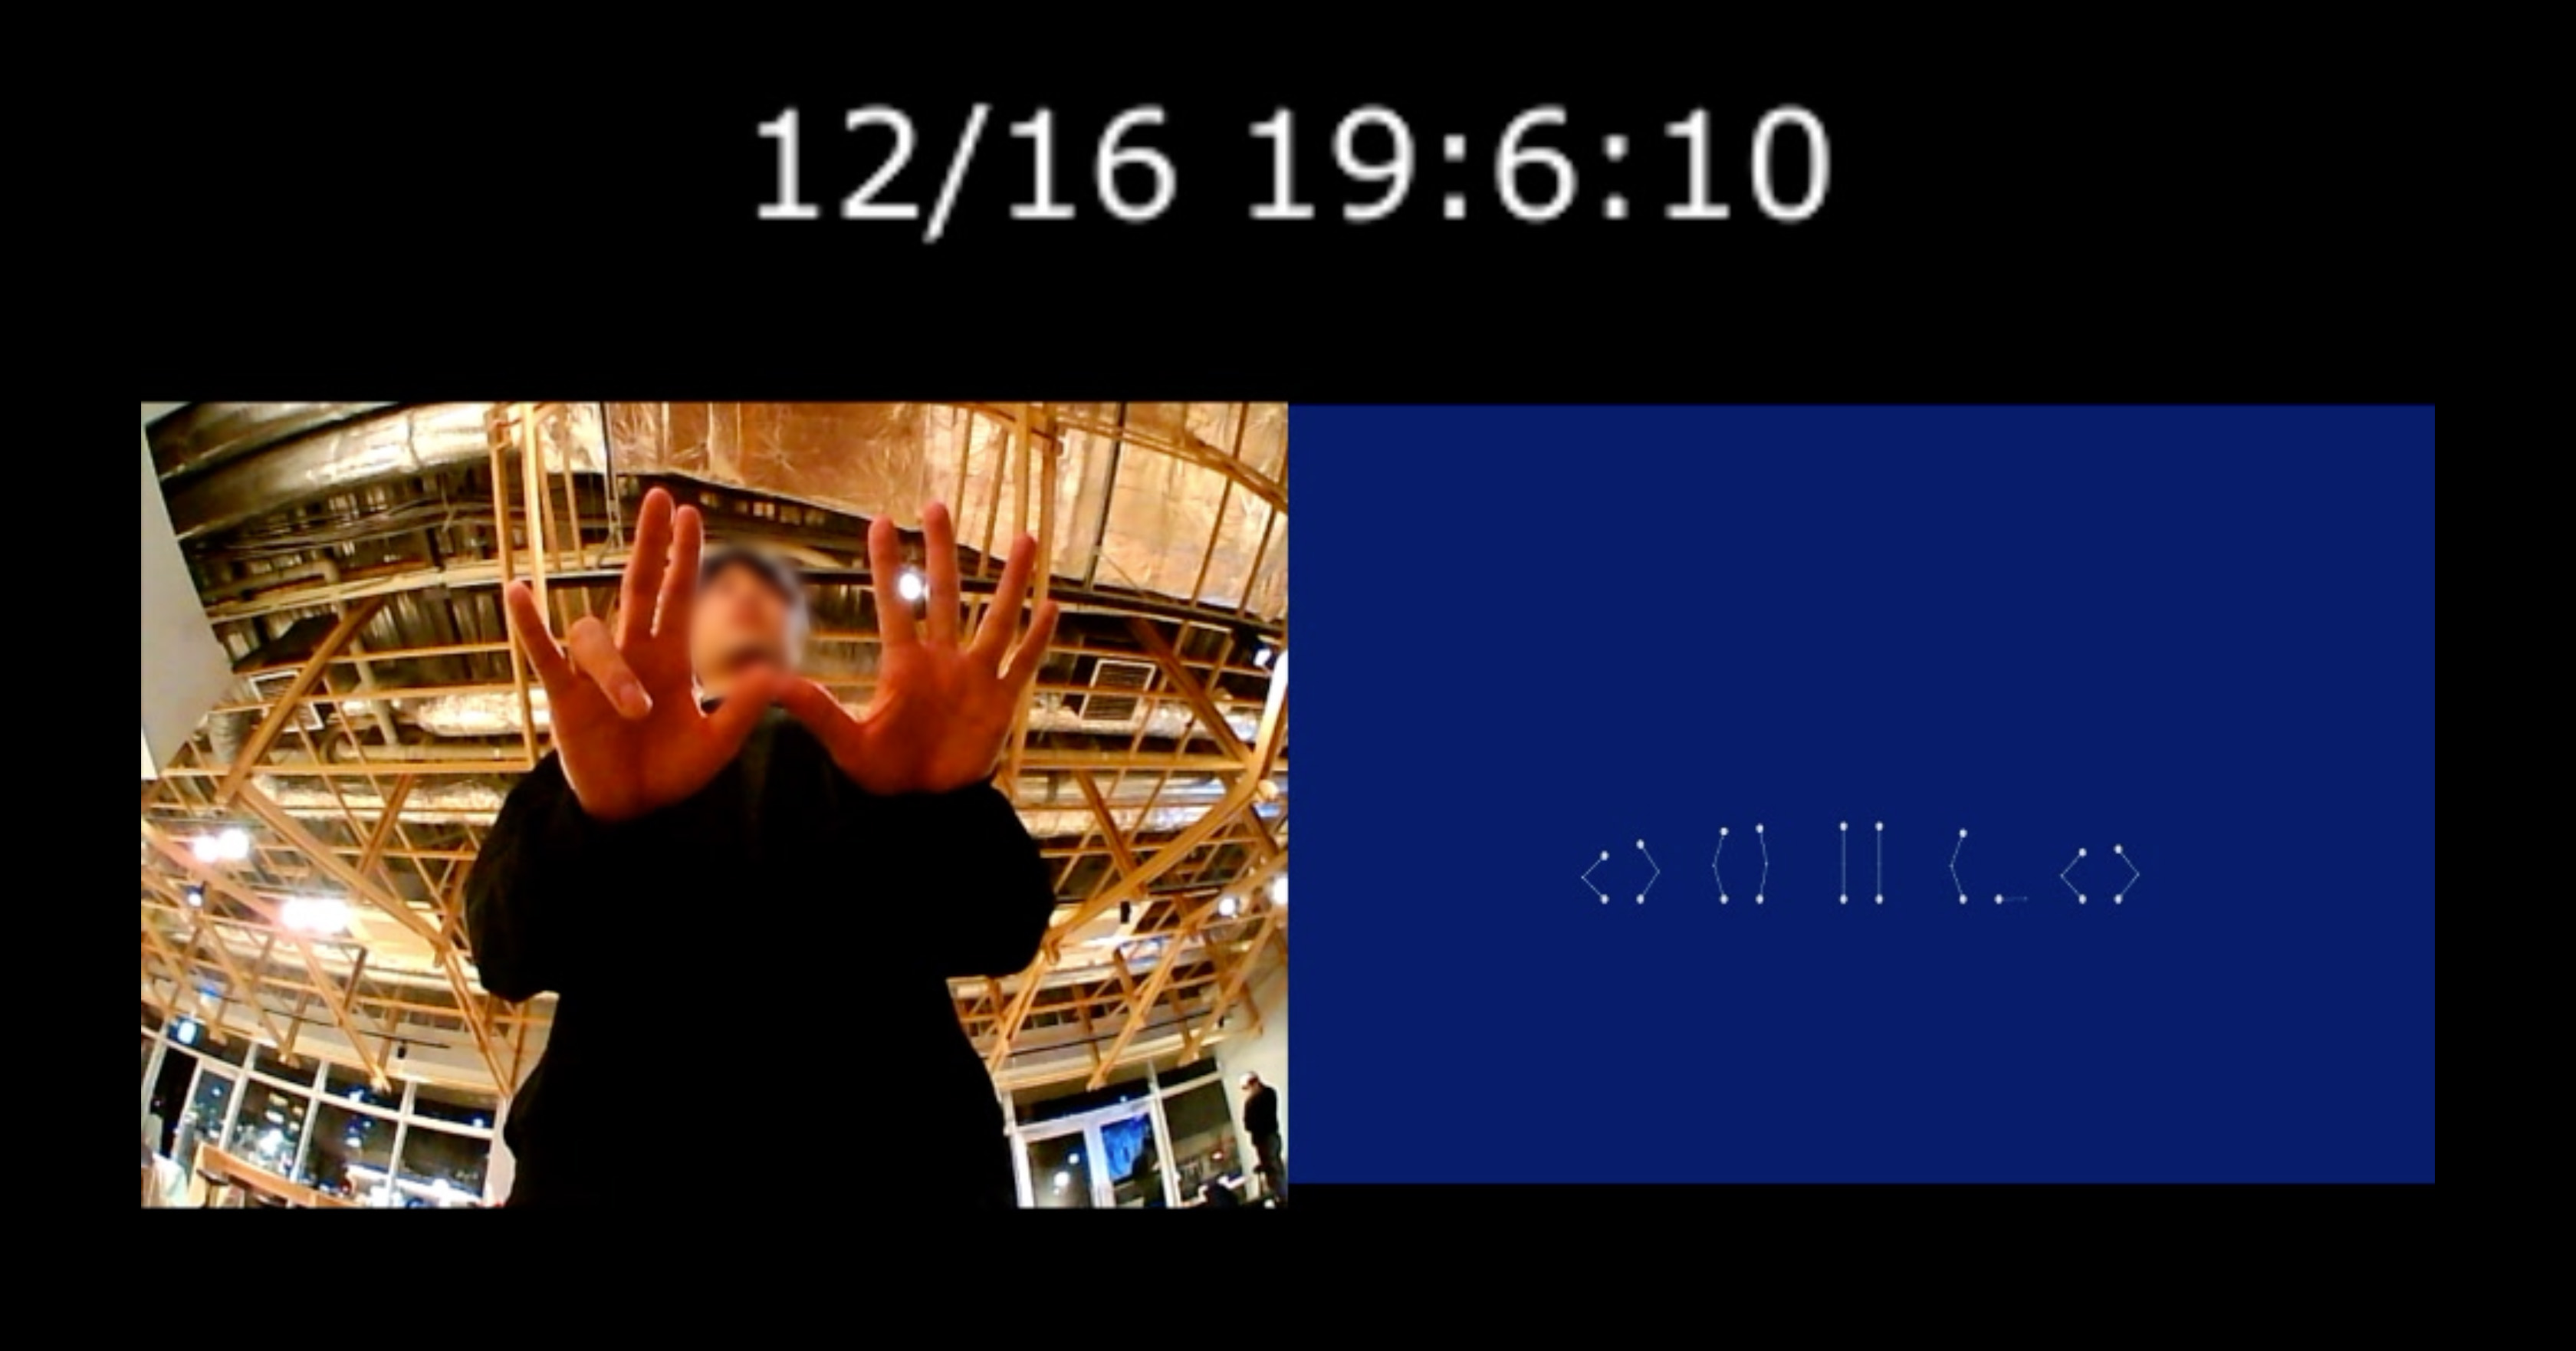
\includegraphics[width=10cm]{img/record_monitor.jpg}
  \caption{体験のようすの記録映像}
  \label{fig:record_monitor}
\end{figure}

作品体験が終了した後、体験者自身が上記の記録映像を視聴しながら、作品体験時のようすを詳細に言語化する振り返り作業を依頼する。この時点では、そのとき考えていたことや、試行した事柄とその理由など、作品体験を終えた今思う感想ではなく、その当時経験していたことについて言語化してもらうよう促した。体験者は、自由に映像を停止したり、巻き戻すことができる。
作業の際は研究実施者も同席しているが、調査を実施する上でのトラブルが生じない限り、原則として体験者個人で振り返る。
その後、前の振り返りの作業や体験のようすを踏まえて、研究実施者が半構造化インタビューを実施することで、より精緻に作品体験のようすを振り返るとともに、体験を終えた上での感想などについて伺った。
いずれもループ構造の作品であるため、1周するまでの期間をその調査対象とした。ただし、作品「Relation」については、一周するための達成条件がシビアであることから、体験の終了は3分以上体験することを目安に、いつでも体験を終了してよいこととした。

\subsection{データの記録}
インタビューから言語化された体験時の回想を、図\ref{fig:spreadsheet}のようにスプレッドシート上に時系列で記録した。シート上には、1秒ごとのタイムスタンプ(日本標準時)、その時刻でのトラッキングの状況(右手、左手、全体)、その時刻での出力内容を示すシーン情報、並びに発言内容が記録されている。また、その後に行ったインタビューについては文字起こしをしてテキストデータで記録した。
\begin{figure}[H]
  \centering
  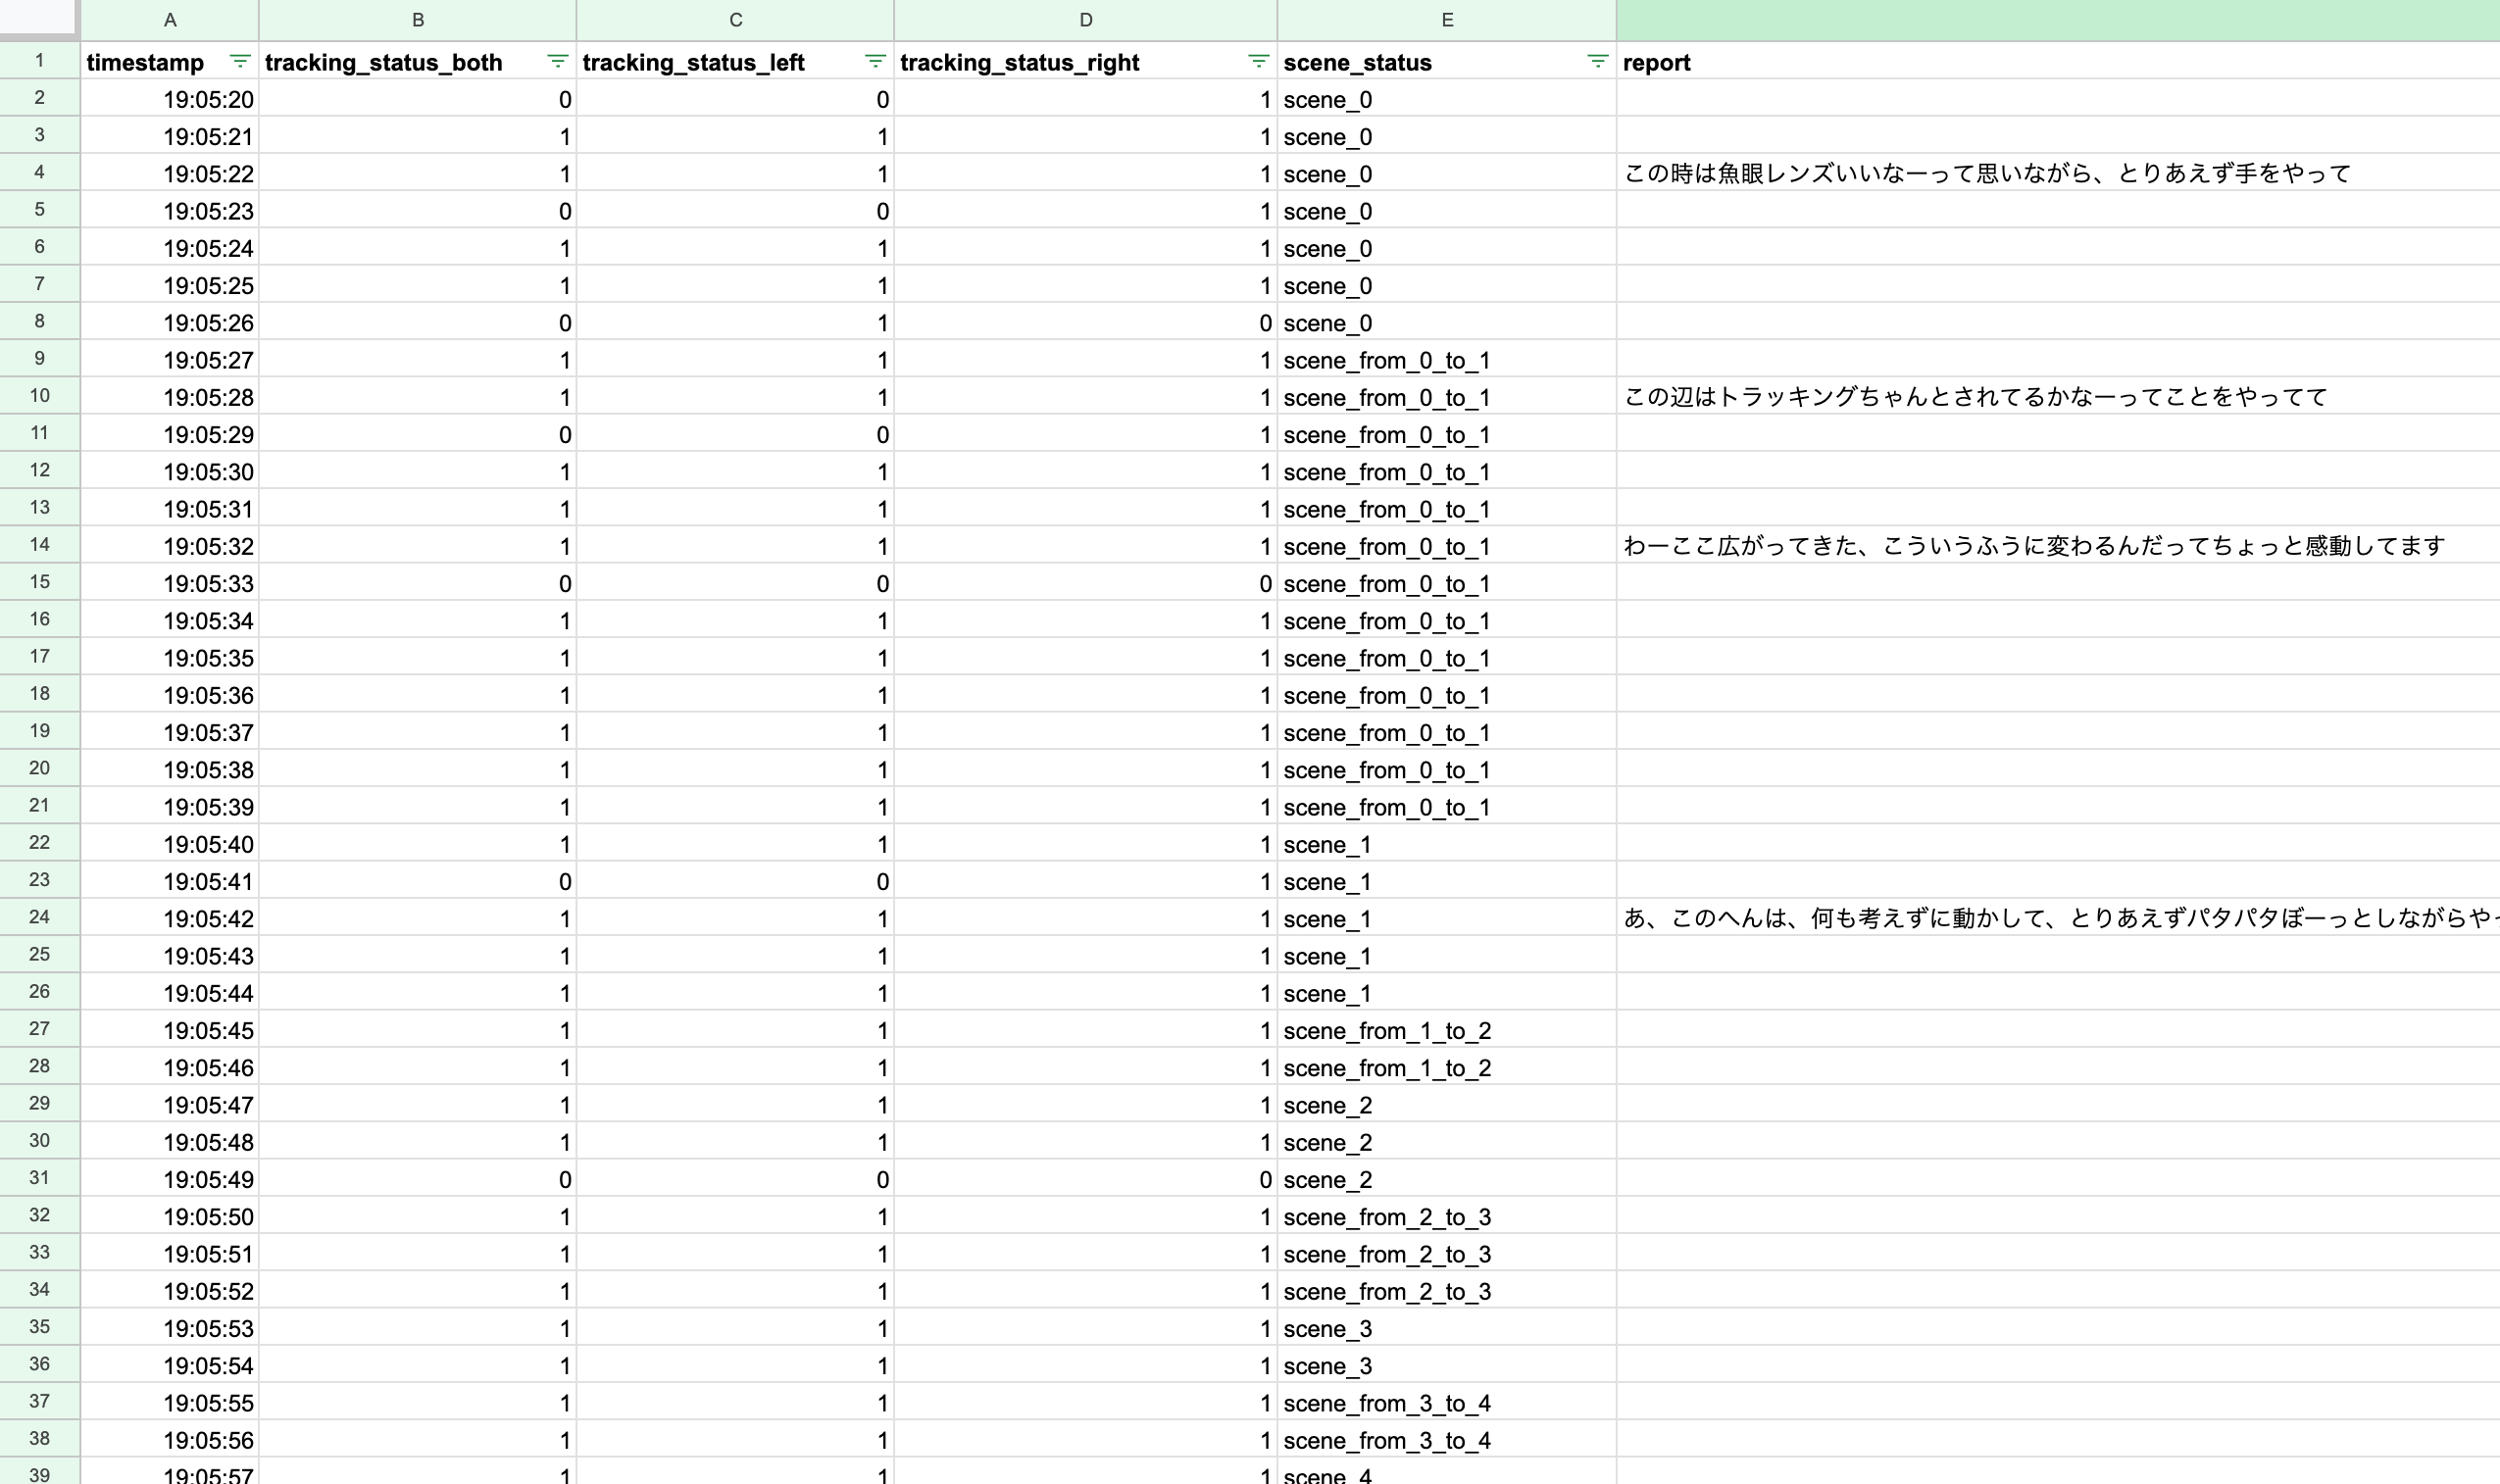
\includegraphics[width=10cm]{img/spreadsheet.png}
  \caption{発話情報が記録されたスプレッドシート}
  \label{fig:spreadsheet}
\end{figure}

\section{結果}
以下では、参加者の体験時の映像とそれをみながら体験者自身が行った回想、そして、インタビューを通して得られた意見から、それぞれの参加者が「Familiar / Strange」、「Relation」をそれぞれどのように体験していたのかについて説明する。

\subsection{Familiar / Strange}
\subsubsection*{参加者1}
参加者1は、シーンが展開していくに連れて徐々に手指の動かし方が変化していった。シーン0からシーン1にかけての、手が指ごとに離れていく過程では、手を握りしめたり、開いたりする動作が見られるが、シーン1以降、関節が減り、左右の指で1セットのまとまりが明確になってくると、指を一本一本曲げる動きをするように変化した。手指の単位で分かれるシーン1からシーン6にかけては、どの指がどの指に対応しているのかについての「確認」を主に行なっていたと語る。
\begin{quote}
  どれがどの場所なんだろうって、最初は手の形になっているのでわかるんだけど、それがずれていってどれがどれかなっていうのを確認してたかな。(参加者1)
\end{quote}
しかしシーン7になると、途端に握り拳を作る動きが多くなる。また、右手と左手を交互に握ったり、指一本単位でも、左右で同じ位置の指を曲げる動きが現れる。体験を振り返って、「干渉するイメージが強くなった」ことについて語る。
\begin{quote}
  今まで二つ単位で独立してたのが全部つながってバネみたいになって、お互いがお互いに干渉するイメージが強くなったかな。全部握ったら、全部閉じるんだ、みたいな。(参加者1)
\end{quote}

また、シーン7からもとのシーン0へと戻る中では、前のシーンでの手の動かし方を受けて、動かし方に変化が見られた。「干渉」構造に気づいた後のシーン7以降も手指の動きに注目すると、前半には少なかった左右の同じ指を同時に動かす動きが増えた。

\begin{figure}[htbp]
  \begin{minipage}[b]{0.5\linewidth}
    \centering
    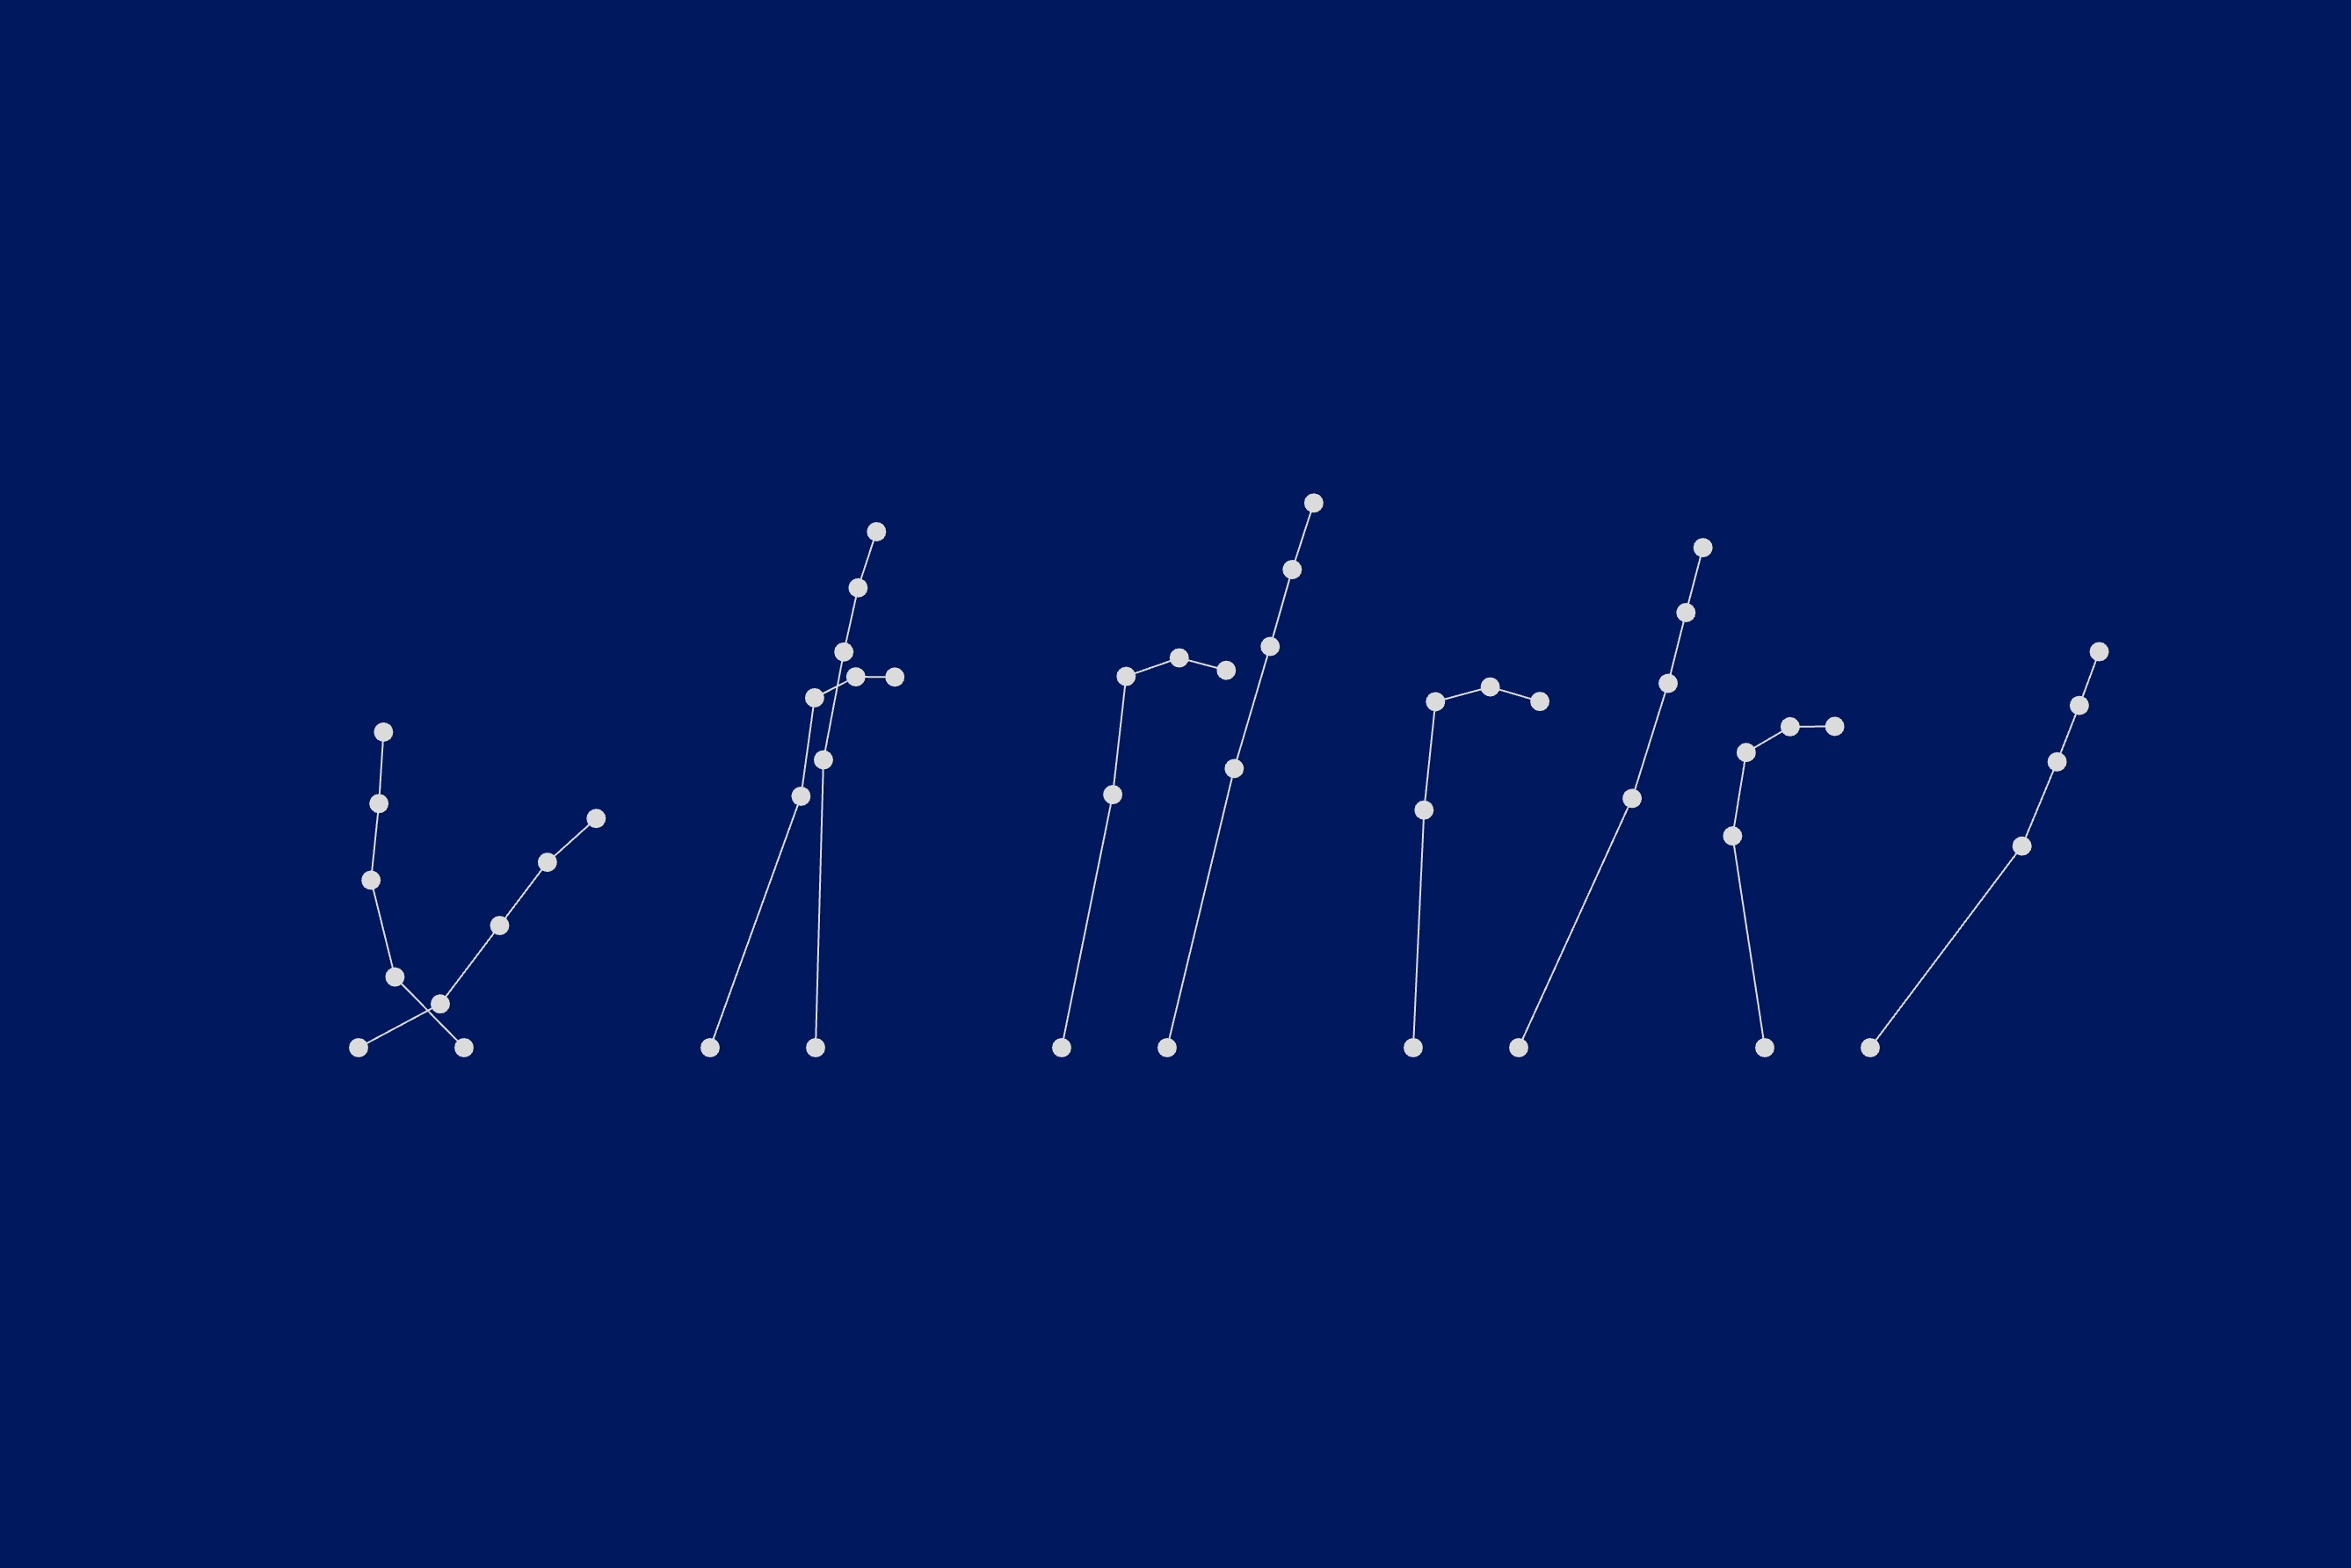
\includegraphics[keepaspectratio, width=7cm]{img/scene1.png}
    \caption{シーン1}
    \label{fig:scene1}
  \end{minipage}
  \begin{minipage}[b]{0.5\linewidth}
    \centering
    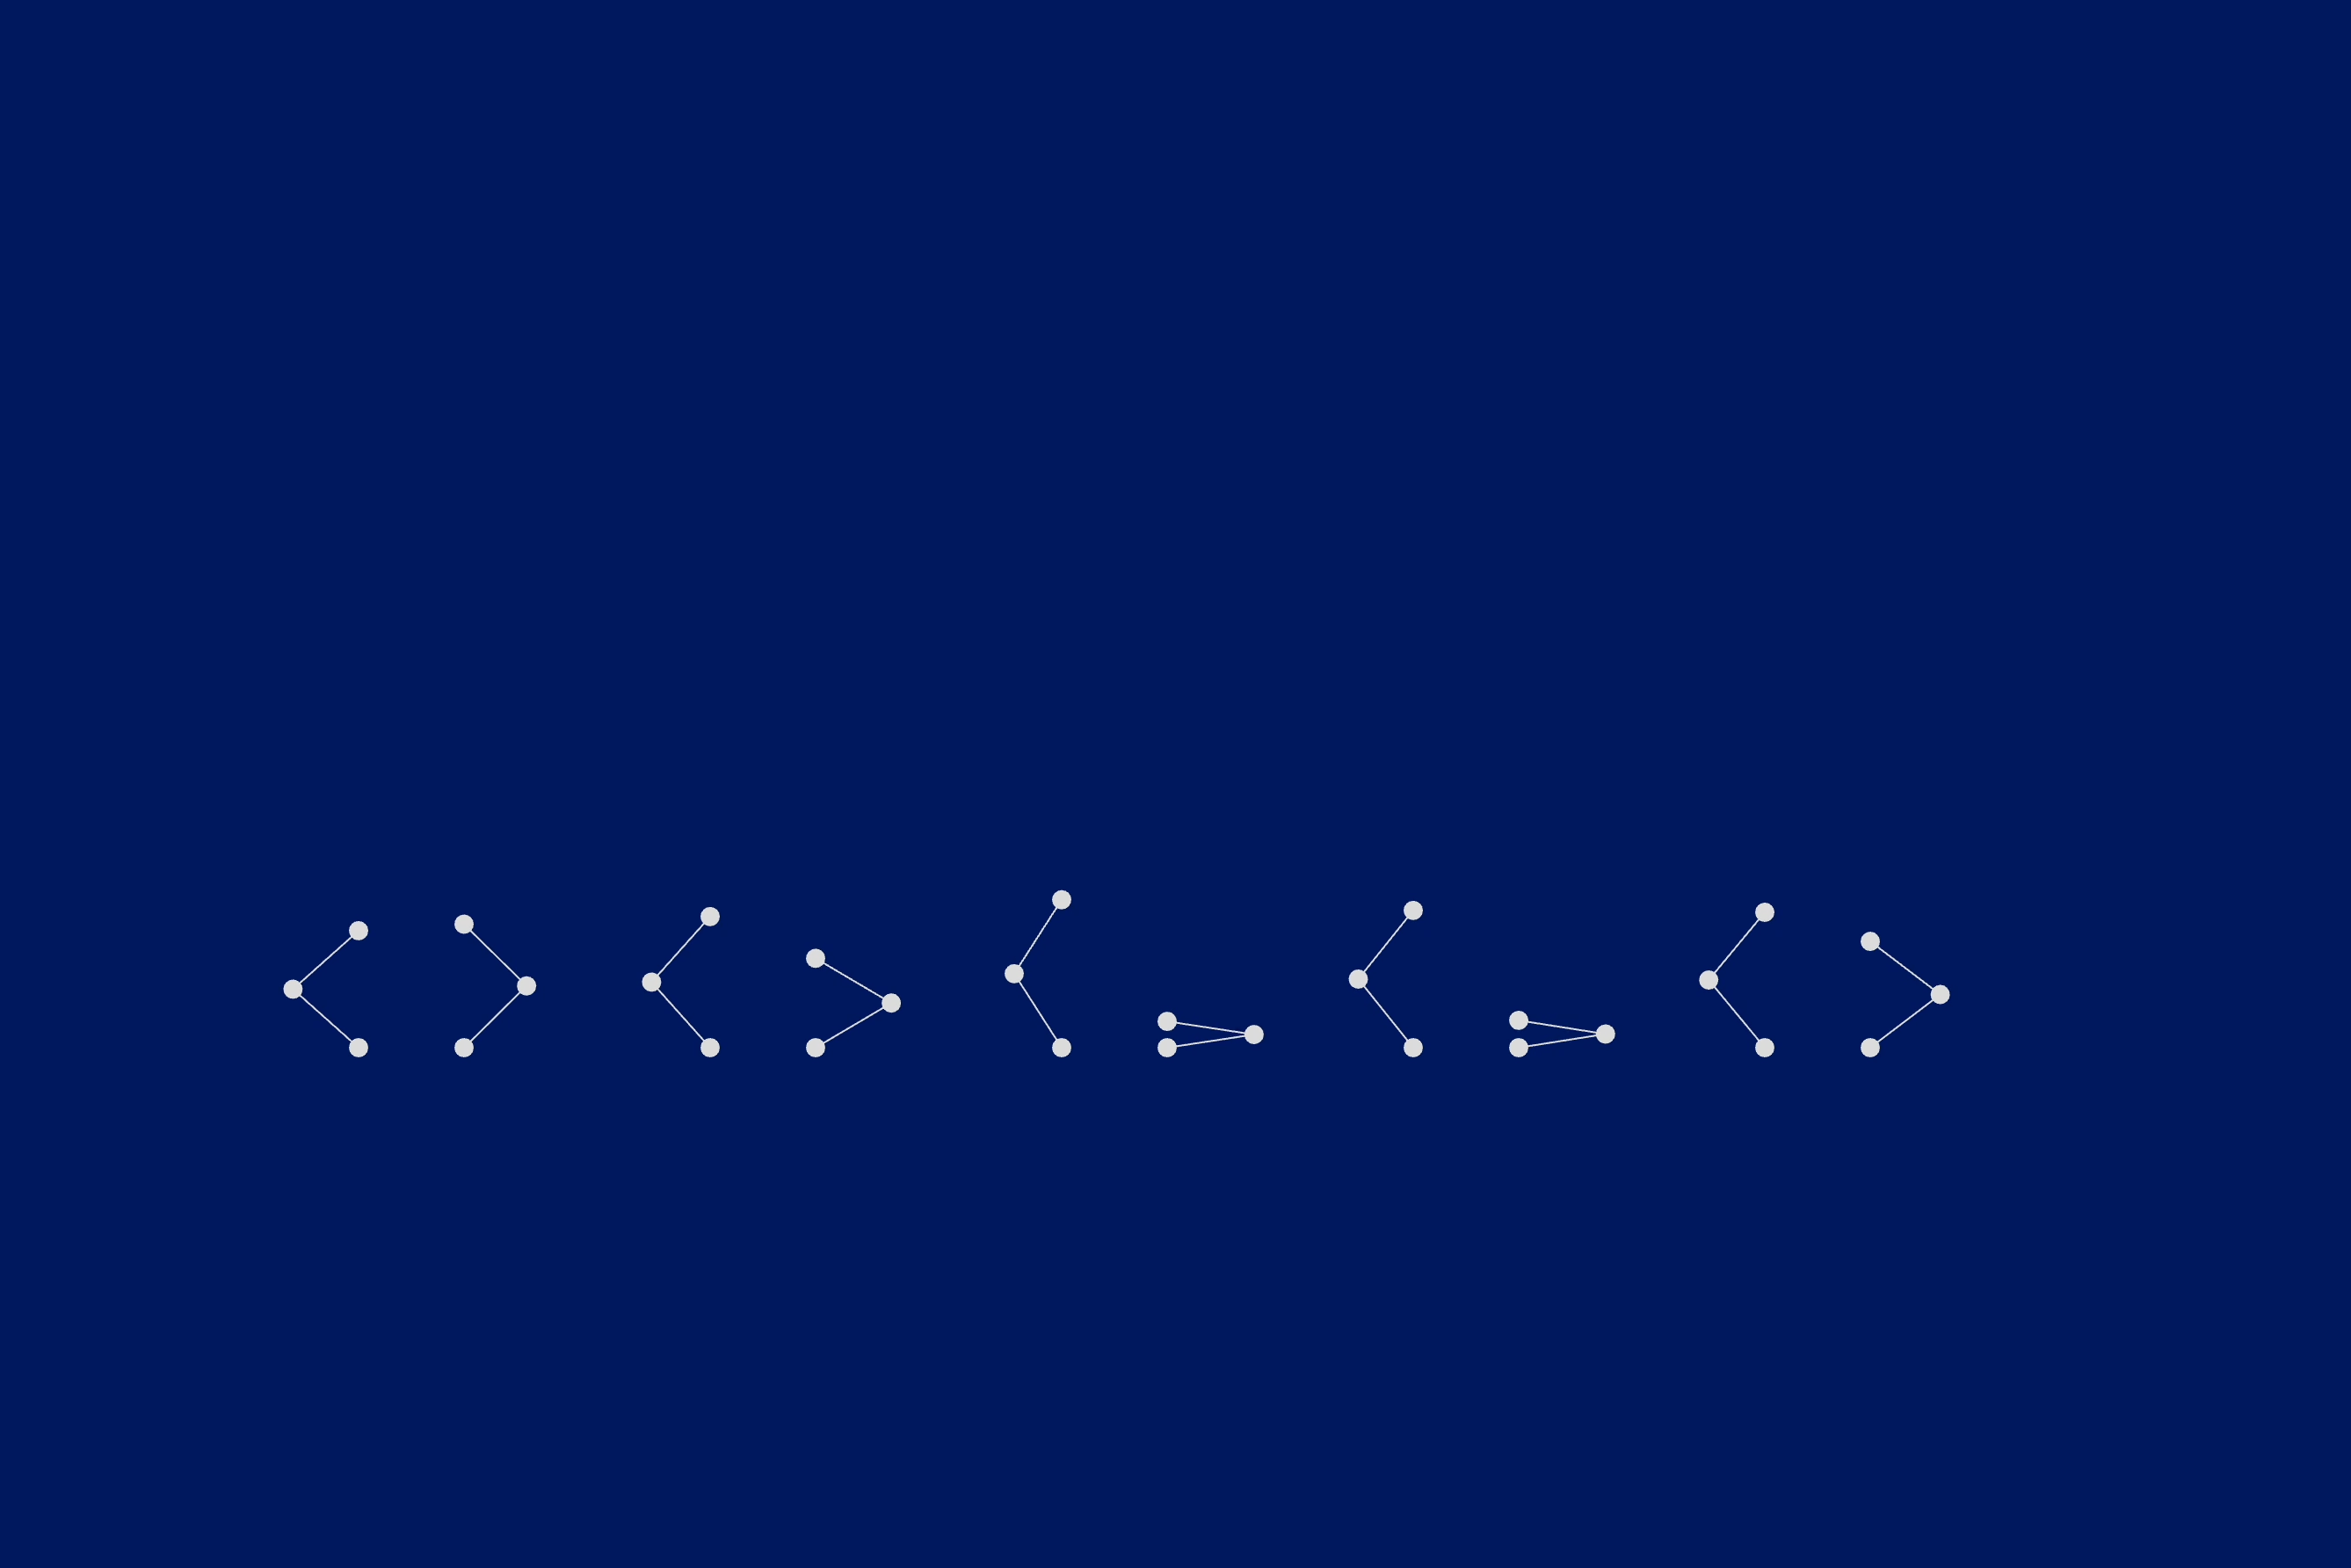
\includegraphics[keepaspectratio, width=7cm]{img/scene6.png}
    \caption{シーン6}
    \label{fig:scene6}
  \end{minipage}
\end{figure}

\subsubsection*{参加者2}
参加者2は、「親和性」という言葉を用いて、体験の中で画面の中の手に対する認識が変化したことについて述べていた。最初、グー、チョキ、パーの形を作って、「自分の手と、モニターに写っている手が、どれぐらい親和性高く動くのか」について確かめていたが、シーン3から4にかけては、「親和性から離れていく感じ」があったと語る。
\begin{quote}
  ここら辺からちょっと違和感というか、親和性を確かめてたのに、その親和性から離れてく感じがしてた。今の自分の手と、こっち側の手の連動はしてるんだけど、離れている。自分の手じゃなくなる。(参加者2)
\end{quote}
そしてシーン7では「親和性」については諦めて、「身体的なところからは離れ」た存在となっていたことを振り返っていた。
\begin{quote}
  ここら辺からちょっと結構激しく手を動かし始めてた。[...]動きの精度を見てる。親和性はもう諦めて、動きの精度みたいなことを、よりシステムチックに見ちゃってる。身体的なところからは離れている、これはもう完全に。(参加者2)
\end{quote}

また、参加者2は特に手指を高速に動かすことで、どのスピードまで反応しうるかについても確かめていたが、そうした高速な動きに対してのフィードバックが強いシーン7では「気持ちいい動き」を「探ってい」たと振り返る。
\begin{quote}
  ここら辺から自分が気持ちいい動きが探っていて。細かい動きを認識するなっていうのがここら辺でわかったから。ただ大きい動きになると、センサーの反応が悪くなったから、気持ちよく動く限りで、細かい微妙な動きをしたり。(参加者2)
\end{quote}

しかし参加者2は、体験の中で「既視感」を作ることが難しい場面については目的意識を見出して体験することの難しさを振り返っていた。
\begin{quote}
  最初のビジュアルが手だったから、もうちょっと「自分の体とシステムの動き」の視点で見てたけど、ビジュアルが変わったことで体験する感覚、意識がそこで変わった。[...]手は見たことある形だったからまだ探る余地があったけど[...]見たことないものになると[...]どうその曲線で遊ぶのかを見つけるのがなかなか大変で。(参加者2)
\end{quote}

\begin{quote}
  でも人の動きとかを[...]解像度高く見るには多分こういう線の方が見やすいと思うんだけど、(一方で)既視感のあるものがここに入ってくるとなんかめっちゃおもろいな。(参加者2)
\end{quote}

\begin{figure}[H]
  \centering
  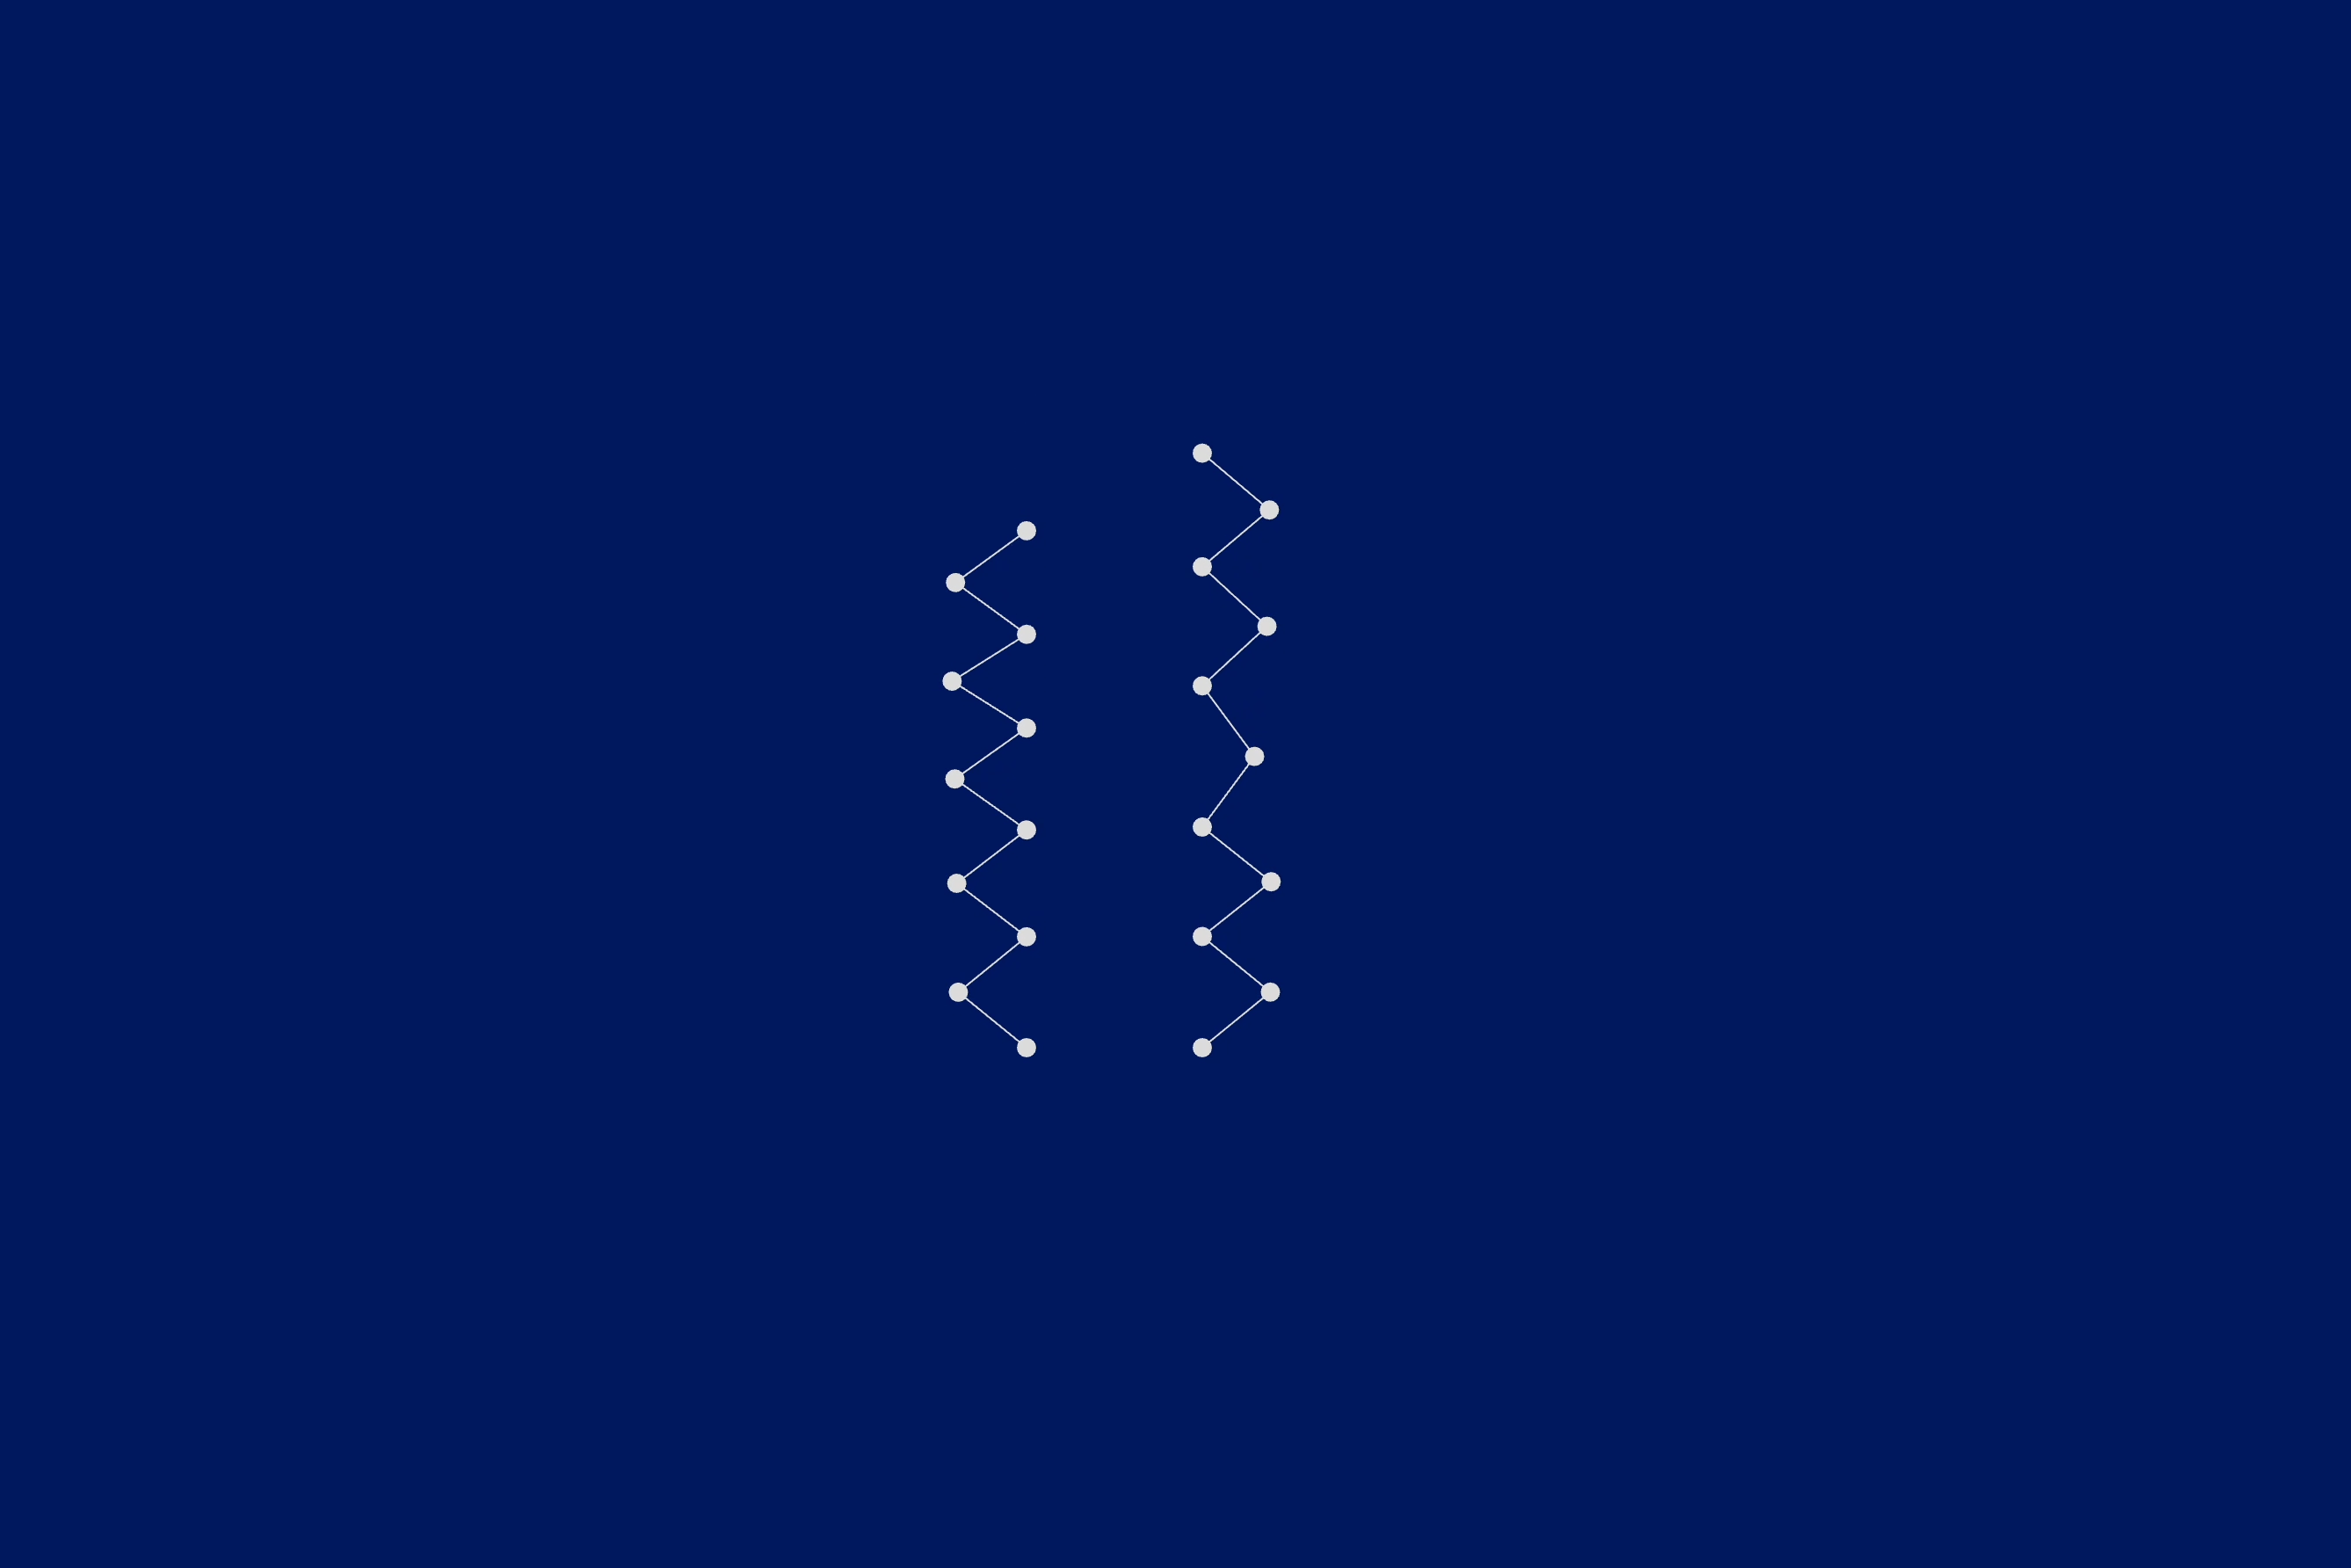
\includegraphics[width=10cm]{img/scene7.png}
  \caption{シーン7}
  \label{fig:scene7}
\end{figure}

\subsubsection*{参加者3}
参加者3は、今回の体験した人は唯一、体験を通して身体の動かし方に変化が起きなかった。最初、フレームを切るようなジェスチャーなどをしていたが、しばらくして自分の動きとは関係なくシーンが遷移していることに気づくと、手を動かすことを止めて「自分が動かなくても動く」ということを確かめていた。参加者3は他の参加者とは違って、指を一本一本動かし、どこがどの指であるかを確かめるような動きは少なかった。シーン3から4に遷移する過程で「こうやってしたら(両手を開いて親指と人差し指をつなげ、三角形を作る)くっつくのかな、みたいなことをやっていました。特にくっつかなかった。」「(指を交差させて)こうやってやったら変わるのかな」と、「形を作る」ことができるのかについて試行していたが、結果「作れなかった」と認識してからは、手を開いた状態で、カメラに手を近づけたり遠ざけたり、手首を回すような動きをとっていた。そして、体験については「途中で飽きていた」と振り返った。インタビューにおいてその理由を尋ねると、「反応が変わらない」ことがその理由であると語った。
\begin{quote}
  関節五個あった時は楽しかったんですよ。それが一個になって、あれ、なんか手を動かしても広げなくても変わらない、やってもやらなくても反応が変わらない。ならやらない、みたいな。(参加者3)  
\end{quote}

\subsubsection*{参加者4}
参加者4は、シーンの遷移に応じて徐々に意識的な身体動作が喚起されていた点について振り返った。最初、手指の動きが認識されたことを受けて、トラッキングがどの程度の精度で認識するのかについて確認していた。シーン0からシーン1にかけての初めての遷移のモーフィングに、「こういうふうに遷移するのかということに、ちょっと感動していた」ものの、シーン1に遷移すると最初、「何も考えずに、とりあえずパタパタと動かしていた」と振り返る。しかし、次第に「自分のどの指に反応してるのかということに気づき始め」、続くシーン4からシーン6にかけては「自分の手の動きと、棒(変換されたくの字のユニット)の動きがどういうふうにリンクしているのか」、「右手と左手の指の位置がどういうふうに対応しているのかを、ちゃんと確かめている」と振り返っていた。また、シーン6では「親指があまり反応していない気がしたから、親指の動きを確かめてい」たと振り返った。これは、身体の構造上、親指だけ屈曲する軸が異なるため、\(y\)軸方向の指先と付け根の距離を評価するこの作品では、身体の動きの量に対するフィードバックが少ないためだと推測できる。また、シーン7に至ると「これはただ気持ちよく動かすことだけを考えていた。気持ちいい動きをしてもらうことだけを考えてた」と振り返り、最初は大きな画面の変化を作っていたが、徐々に「冷静になって、どんなメカニズムになっているのかを探り始め」、指を動かすだけでなく、画面に対する手指の向ける角度を変える動きを試みるなどして、シーン7からシーン6に差し掛かるあたりで「思い通りに動かせる」と感じていたことを振り返った。再びシーン5からシーン1にもどる過程では、これまで指の動きだけに限定されていたことに気づき、それだけではない、距離や角度、手首の高さなど様々な動きについて検証し始めたと話していた。

しかし、参加者4は体験の中で、たびたび「何も考えていなかった」瞬間について言及しており、それらはトランジションのタイミングに集中していた。具体的には、シーン0からシーン1へのトランジションの最中、シーン6からシーン7へのトランジション、再びシーン1からシーン0へのトランジションである。

\subsection{Relation}
\subsubsection*{参加者1}
参加者1は最初、マトの存在には気づかず、「左にボールがあったら右の方に移動させようとか、右にあったら左に移動させてみよう」と、左右にボールを移動させることについて目的意識を持って、球を操ろうと試みていた。しばらくすると、ボールが偶然球にあたり、それからマトに当てることを目指すようになった。これについては、「ちゃんと当てようと思ってたんだけど、なかなか当たら」なかったと振り返る。\\
手指の動きに注目すると、マトに当てることを目指すようになってからは手指の動かし方には大きな変化が見られなかった。途中、マトの方に向けて手をはらうような動きをしてみたり(17:31:05)、手のひらを裏返した状態で動かそうと試みる(17:31:08)が、思うような挙動はしなかったためか、手指の姿勢は元の姿勢へと戻った。
\subsubsection*{参加者2}
参加者2は、途中までマトの存在に気づかないまま体験していた。その中で、ボールの投げ上げに「どれぐらいの動きでどれぐらいバウンドするのか」、「ボールをちょっと滞在させたい」「ちょっとなだらかな面を作ろう」とする、波打つような動きを作るなど、マトに当てるということ以外での目的設定をしながら身体を動かしていた。途中、
\begin{quote}
  ちょっとコツを掴もうと思って、一回動きを静かにして、動きのコツを探してたけど、なかなか難しくて。左に投げたいのに、左にあまり流れない、みたいな。角度傾斜をつけて、ある程度投げたい位置まで来たら、上にあげたらいいんじゃないかなっていう。無理くり、投げる角度でコントロールするのは難しいな、と。  
\end{quote}
と、投げ上げに関して「コツを掴もう」としたことについても振り返っている。しかし一方で、ボールを投げ上げてマトに当てるということに目的意識が芽生えてからは、波打つような動きを作るときとは違って「イライラ」していた感覚について語っている。その理由として「反応の鈍さ」に言及する。
\begin{quote}
  投げるときの反応が鈍くて、ちょっとイライラしてた。前の手のトラッキングだけとは違って、線が入ることで、もどかしいっていうか。  
\end{quote}
\subsubsection*{参加者3}
参加者3はボールの出現に際して「トランポリンみたい」(13:06:14)だという見立てから、高く飛ばしてみるということを試みていた。その後、ボールが画面の端から転がり落ちた(13:06:22)ことを確認して、「落ちるのは良くなさそう」と捉え、「次からは落とさないようにしよう」と制約をかけるようになった。さらに、高く飛ばしたボールが偶然マトに当たることを繰り返す(13:06:19 / 13:06:21 / 13:06:36)中で、「そうかあれは当てればいいのか」と認識し、マトに当てることを目的として設定するようになった。手指の対応関係については、端から小指、中心に両手の親指となる順で並べられているという構造については認識していたと振り返る一方で、体験の途中では手のひらを上に向け、掬い上げるような動きをしてボールを投げ上げる動きを試みていた。
しかし、しばらく当たらない状態が続き、諦めて体験が終了した。

% \subsection{全体的な感想について}
% \subsubsection*{参加者1}
% (執筆中)
% \subsubsection*{参加者2}
% (執筆中)
% \subsubsection*{参加者3}
% (執筆中)
% \subsubsection*{参加者4}
% (執筆中)